This section details the implementations proposed by the paper. This includes two Software Transactional Memory versions and transactional Red-Black Tree and Skiplist datastructures, which are used to benchmark and evaluate the performance of said STMs; moreover, they demonstrate the ease of designing transactional algorithms. 

\section{Software Transactional Memory}
\label{subsec:stm_impl}

The lock-based Software Transactional Memory versions are implemented in C++ and they have the following interface which can be seen in Figure \ref{fig:interface}, that all implementations override. Upon creating a transaction \texttt{Tx}, \texttt{Tx.begin()} takes care of initialising its internal state. \texttt{Tx.commit()} attempts to commit the transaction and returns \texttt{true} if it succeeded and throws an \texttt{AbortException()} if it didn't. In the latter case, the transaction can be retried. \texttt{Tx.abort()} resets the transaction, clears its logs and, in case of an \textit{encounter-order} transaction, rolls all writes back. \texttt{Tx.read(T *addr)} transactionally reads the value of the pointer \texttt{addr} and returns it, while \texttt{Tx.write(T *addr, T val)} transactionally writes in place of \texttt{addr} the value \texttt{val}.

\begin{figure}[!htb]
\centering
\label{fig:interface}
\begin{tabular}{c}
\begin{lstlisting}[language=C++]
template<class T>
struct Transaction {
    virtual void begin()       = 0;
    virtual void write(T *, T) = 0;
    virtual T    read(T *)     = 0;
    virtual bool commit()      = 0;
    virtual void abort()       = 0;
};
\end{lstlisting}
\end{tabular}
\caption{Transactional interface}
\end{figure}

In pseudocode, statements that need to execute atomically are usually denoted with an \texttt{atomic \{...\}} block wrapping the instructions. Provided that compiler support exists for such a block, it could be parsed the following way: each \textit{read} operation in the form \texttt{int a = *b;} is replaced by \texttt{int a = Tx.read(b);} and each write operation in the form \texttt{int b = 42;} is replaced by \texttt{Tx.write(\&a, 42);}. Moreover, the atomic block needs to be able to repeat itself after seeing an inconsistent state and aborting. This is facilitated by a \texttt{try-catch} block nested inside a \texttt{while} loop. This code structure can be seen in Figure \ref{code-structure}.

\begin{figure}[!htb]
\centering
\begin{tabular}{c}
\begin{lstlisting}[language=C++]
Transaction Tx;
bool done = false;
while (!done) {
    try {
        Tx.begin();
        
        /* atomic block */
        
        done = Tx.commit();
    }
    catch (AbortException&) {
        Tx.abort();
        done = false;
    }
}
\end{lstlisting}
\end{tabular}
\caption{Transactional code structure}
\label{code-structure}
\end{figure}

The rest of this subsection details how transactions maintain consistent states through \textit{ownership records}. Afterwards, the two proposed approaches to performing transactions is presented, which differ in terms of their lock-acquisition approach: one performs \textit{encounter-order}, while the other performs \textit{commit-time} locking. The implementations and their details are presented through how the algorithms override the \texttt{Transaction<T>} interface in Figure \ref{fig:interface}.

\subsection{Ownership Records}
When a transaction wishes to access a location for reading or writing, it first fetches the location's \textit{ownership record (orec)} or \textit{versioned write-lock}, as it is also described in \cite{tl, tl2, book}. Ownership records are a word in memory, which have two distinct states. When unlocked, the ownership record's lowermost bit is $0$, and the rest of the bits represent the \textit{version} of the object it references. Before writing an object, each transaction must acquire the record while ensuring that the object's version didn't change in the meantime. This can be achieved by an atomic \textit{CAS}. When locked, the ownership record's lowermost bit is $1$, while the rest of the bits represent the ID of the transaction. To unlock the record, its lowermost bit is cleared, while the rest of the bits store an increment of its previous version. Since every location in memory cannot be associated with a unique ownership record (since there would be too many), a many-to-one mapping is utilised to fetch the corresponding record. This is also called \textit{lock-striping}\cite{tl, tl2}.

\begin{figure}[!htb]
    \centering
    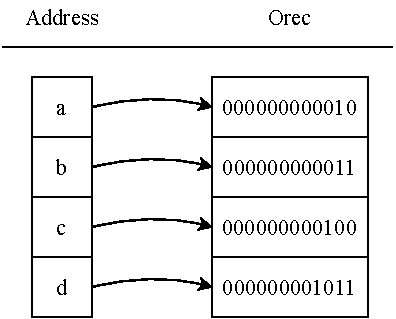
\includegraphics[width=.5\textwidth]{images/orec.pdf}
    \caption{Addresses in memory with their associated orec. Address $a$ is unlocked with version 1, Address $b$ is locked by Transaction nr. 1, Address $c$ is unlocked with version 2, and Address $d$ is locked by Transaction nr. 5}
    \label{fig:orec}
\end{figure}

\subsection{Encounter-order Transactions}
\label{subsection:etx}
Encounter-order or \textit{direct-update} transactions modify transactionally accessed memory directly. Between the transaction begins and tries to commit, all reads and writes are performed while keeping transaction-local \textit{read}, and \textit{undo} sets. The read set is used to validate during the execution of the transaction that all read-only locations' current version matches with the version recorded in the read set. The undo is used to roll back the writes upon aborting and restore the original values.

When encountering a transactional read, the location's \textit{ownership record} is fetched. The transaction needs to first check whether it already holds the lock, and in that case, the location's value can be atomically loaded, while the current version of the object is stored in the transaction's read set. In case the transaction does not hold the associated lock, it checks whether some other transaction does. If it finds the location to be locked, it can either spin or abort and retry. If the location is not locked, the value can be atomically loaded, while the current version of the object is stored in the transaction's read set.

In the case of a transactional write, firstly, the ownership record associated with the address is fetched. The transaction then must acquire the record in order to ensure that only a single transaction can write to the same location. If the lock could not be acquired (because another transaction successfully acquired it in the meanwhile), the transaction aborts. If the transaction acquired the lock, or it already holds the record, the address' current value is saved in the transaction's \textit{undo} set, and the new value is atomically stored at the address.

During the execution of the transaction, the read set must be validated to ensure that the recorded versions match the objects' current version. If a mismatch is found, there is a \textit{read-write} conflict between two transactions. In that case, another transaction modified the object that the transaction previously read; therefore, the transaction with the invalid read-set must abort.

When committing, the transaction revalidates its read-set, and if it is found to be valid, releases all locks and returns. The transaction is now considered to be committed.

Upon aborting, the transaction uses its undo-set to roll back all writes and restore the previous state as if nothing had happened. Then, it can choose to retry immediately or utilise some form of back-off, which might be useful in case of high contention.

The encounter-order approach, similar to the approaches of \cite{tl,ennals-stm}, makes committing much simpler. However, encounter-order locking has the downside of holding onto locks for a much longer time, potentially hindering performance under high contention.

\subsection{Commit-time Transactions}
\label{subsection:ctx}
Commit-time or \textit{deferred-update} transactions utilise a higher level of \textit{speculative execution} by deferring writes to commit time. During the execution, a \textit{write-set} is built, which stores the to be written values. Naturally, a \textit{read-set}, consisting of read locations and their current value, is also being book-kept, which ensures that the transaction sees valid states only.

A transactional read of an address first needs to check whether the address appears in its write-set as well, and in that case, return the latest new value in the write set. If the write set does not contain the address, the associated ownership record is fetched. If the location is found to be locked, the transaction can spin or abort. Else, the current version of the object is stored in the transaction's read set, and the location is atomically loaded.

All transactional writes are deferred to commit time; therefore, performing writes amounts to recording the address-value pair in the transaction's write-set.

During the execution of the transaction, the read-set is validated periodically by checking that the recorded version of objects matches the current version. If the read-set is found to be invalid, the transaction aborts.

When committing, all locks associated with entries in the write set must be acquired. This is done as follows: if a location in the write set appears in the read set as well (i.e. the transactional write depended on the read or vice-versa), the operation must atomically acquire the lock and validate that the version of the object at hand did not change during the execution of the transaction. If the location does not appear in the read set as well, the transaction simply acquires the associated locks. In case a lock cannot be acquired, the transaction aborts. Once all locks are acquired, the read-set is revalidated to ensure consistency, and finally, all updates are made visible using atomic stores. Afterwards, all locks are released, and the transaction is considered to be committed.

When aborting, the transaction must release all previously held locks and can be retried or can back-off based on contention.

The commit-time approach, similar to the approach of \cite{tl} and as also discussed in \cite{tl, tl2, book}, presents a much easier write operation; however, due to its speculative nature, committing is much harder, and reading involves a look-aside into the write set. For the latter, fast approaches using \textit{Bloom filters} exist, as discussed in \cite{tl2}.

Moreover, as will be presented in the Results section, commit-time transactions have an inherent limitation due to the way writes are handled. That is, only those writes will correctly be made visible, which do not depend on \textit{previous} transactional writes. In the case of transactional red-black trees, inserting a node relies heavily on intermediate rotations and recolourings, which makes commit-time transactions unsuitable or the datastructure design unnatural. In the case of skiplists, the problem disappears since swinging pointers at a certain level does not depend on earlier computed results. 

\FloatBarrier
\section{Transactional Red-Black Trees}
\label{section:trb}

One of the custom datastructures is a transactional Red-Black Tree implementation that is used to evaluate the performance of the proposed STM versions and demonstrate the ease of transactional datastructure design.

\textit{Binary trees} are tree-graphs with a root in which each node has at most two children. A \textit{binary search tree} (or BST for short) is a type of search datastructure built on top of binary trees. In a BST, each node is an object that contains \texttt{left-child}, \texttt{right-child} and \texttt{parent} pointers to other nodes, and a \texttt{key} attribute. Keys are stored with the condition that each node's key must be larger than any key in its left subtree and smaller than any key in its right sub-tree, or in other words, flattening the tree gives an increasing sequence of keys. In a binary search tree, the operations of search, insertion and deletion run in $\mathcal{O}(\text{log n})$ time in the average case; however, in the worst-case, these datastructures offer no greater performance than linked-lists with $\mathcal{O}(n)$ time\cite{introalg}. The reason behind this is that BSTs do not \textit{balance} themselves after the tree is modified; therefore, successive insertion of strictly smaller or larger elements will result in a linked-list-like structure starting at the root, which can be seen in Figure \ref{fig:bst}b.

%\renewcommand{\thefigure}{1a-1b}
\begin{figure}[!htb]
    \centering
    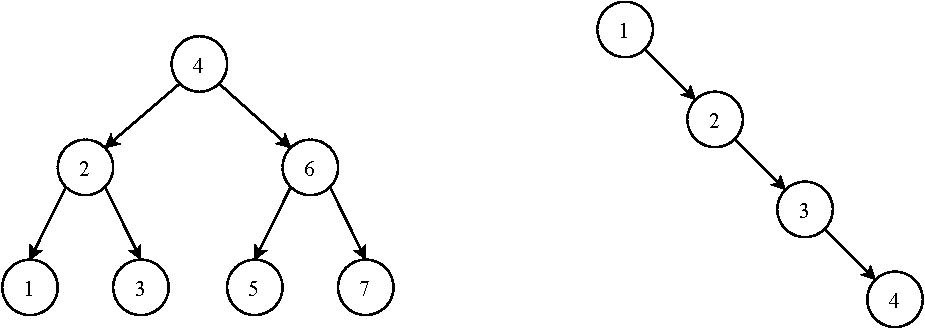
\includegraphics[width=.9\textwidth]{bst.pdf}
    \caption{a) balanced BST b) unbalanced BST}
    \label{fig:bst}
\end{figure}

Red-Black trees are a type of \textit{self-balancing} binary search tree that aim to solve the previously mentioned performance issue, permitting $\mathcal{O}(\text{log n})$ worst-case search, insertion and deletion complexity\cite{introalg}. A binary tree is considered to be balanced if the height of each nodes' left and right sub-tree differ by no more than one. The height of a binary tree is defined as the length of the longest possible path from the root to a leaf node (i.e. a node with no children).

\begin{figure}[!htb]
    \centering
    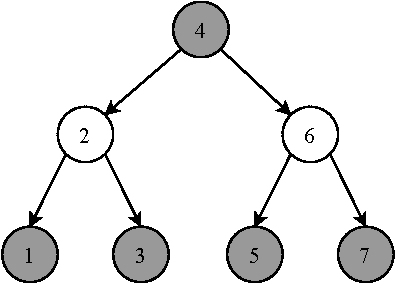
\includegraphics[width=.4\textwidth]{rbt.pdf}
    \caption{A red-black tree with shaded black and unshaded red nodes}
    \label{fig:rbt}
\end{figure}

In a red-black tree, compared to binary search trees, each node has an extra attribute, its \texttt{colour}. Each node is coloured either red or black, which, along with some local \text{rotation} operations, ensure that the tree remains balanced after insertion and deletion. The tree is painted in such a way that the following properties hold\cite{introalg}:

\begin{enumerate}
    \item Every node is painted either red or black
    \item The root and leaf nodes are black
    \item Every red node's children must be black
    \item From each node to its descendant leaves, all paths contain the same number of black nodes
\end{enumerate}

In binary search trees, the root's parent and the leaf nodes' left and right child pointers point to \texttt{NIL} (i.e. to nothing). By convention, in a red-black tree \textit{T}, a single sentinel node \textit{T.nil} is used to represent pointers to \texttt{NIL} which is always coloured black. This node has the same properties as any other node in the tree but with arbitrary key and left-right pointers. This implies that the leaf nodes of a red-black tree are always a single sentinel node; moreover, that the second part of property (2) is always ensured.

Inserting a key into a binary search tree can be summarised as follows. Start at the root of the tree and perform the following until the current node pointer is \texttt{NIL}: if the current node pointer is \texttt{NIL} insert the node at that position. If the current node is not null and the key we wish to insert is smaller than the current node's key, move the current node pointer to the left; else, move it to the right. This algorithm modifies the tree structure, which may or may not violate the properties of a red-black tree. These properties, which might be violated, are namely that the root needs to be black and that a red node cannot have red children. Therefore, when inserting keys into a red-black tree, the tree may need to be repainted, and the tree structure may need to be modified. Modifying the tree structure relies on local \textit{rotations} which are illustrated in Figure \ref{fig:rotate}.

\begin{figure}[!htb]
    \centering
    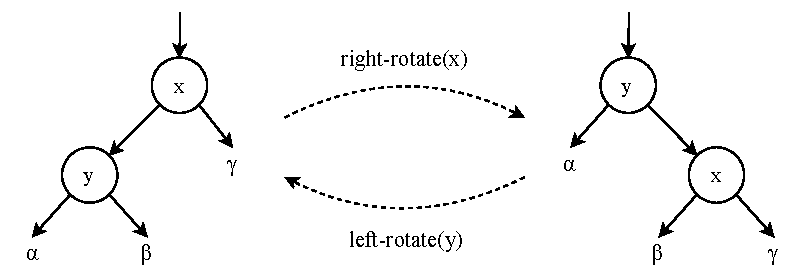
\includegraphics[width=.9\textwidth]{rotate.pdf}
    \caption{Rotation operations on binary search trees}
    \label{fig:rotate}
\end{figure}

One promising aspect of transactional datastructure design and one reason for choosing red-black trees is the simplicity involved in crafting them compared to the lock-based or lock-free approaches. Inserting and deleting keys in a red-black tree involves a \textit{rebalancing} or \textit{fixup} method compared to simple binary search trees, which makes the number of local rotations needed not known in advance. The lock-based approach would have difficulties creating a cycle-free acquisition order\cite{book}, and a lock-free approach\cite{ma, lock-free-rb, wait-free-rb} would involve modifying multiple locations at once. With transactions, the complexity of crafting such datastructure reduces to merely specifying which method needs to execute atomically, and the runtime environment will take care of the rest, which, arguably, also makes the process of crafting such datastructures more accessible and less prone to mistakes. 

To demonstrate the simplicity regarding transactional datastructure design, consider as an example the insertion algorithm described in Algorithm \ref{alg:insert}, and its transactional translation in C++ in Figures  \ref{fig:tx_insert}. The algorithm, which inserts node $z$ with key $k$ into a red-black tree $T$, can be roughly summarised as follows, while, for the sake of simplicity, the description of the fixup method responsible for repainting and performing rotations on the tree is omitted. Firstly, pointers $y$ and $x$ are initialised to nil and the root of the tree in this order. While $x$ does not point to nil, $y$ is swung to $x$ (this pointer keeps track of the parent of the new node $z$), and based on the new node $z$'s key, $x$ is swung either to its left or right child pointer. After the location of the new node is found, its parent pointer is assigned $y$. If the parent pointer is still nil, the tree was empty; therefore, the root is assigned the new node. If the tree was not empty, depending on the key of $z$, the parent node's left or right child is assigned $z$. Finally, the new node is initialised with nil left and right child pointers and the colour red.

In order to "transactionalise" this algorithm, one would need to specify which lines should execute atomically. In pseudocode, this is usually marked as an \texttt{atomic \{...\}} block wrapping the statements in the method. Provided
that compiler support exists for such, the atomic block would be parsed with a transaction initialisation in the beginning and \textit{read} statements in the form \texttt{int a = *b;} replaced with \texttt{int a = read(b);} and \textit{write} statements in the form \texttt{A = b;} replaced with \texttt{write(\&A, b);}. Here, the functions \texttt{T *read(T *)} and \texttt{void write(T *, T)} refer to the transactional interface described in Section \ref{subsec:stm_impl}. Such a translation of the sequential method can be seen in Figure \ref{fig:tx_insert}.

The method \texttt{void tx\_rb\_insert(Node<T> *)} is a member of the class\\ \texttt{TransactionalRBTree<T>} and operates on pointers to \texttt{Node<T>} objects. Notable differences to Algorithm \ref{alg:insert} are line 2 which set up a new transaction as described in Section \ref{subsec:stm_impl}, line 6 which starts the transaction, and line 29 which commits it. The atomic block (i.e. statements that should execute atomically) is placed in a \texttt{try-catch} block which is retried until the transaction is able to commit. All reads are replaced by a method calls to \texttt{Tx.read()} and writes are replaced by calls to \texttt{Tx.write()}. In case the transaction fails, i.e. during the insertion procedure some inconsistencies are encountered, all methods throw an \texttt{AbortException} which is caught by the \texttt{catch} block. The transaction then aborts itself and is retried.

\begin{algorithm}
\caption{RB-Insert(T, z)}
\label{alg:insert}
\begin{algorithmic}[1]
    \State y $\gets$ T.nil
    \State x $\gets$ T.root
    \While {x $\neq$ T.nil}
        \State y $\gets$ x
        \If{z.key $<$ x.key}
            \State x $\gets$ x.left
        \Else 
            \State x $\gets$ x.right
        \EndIf
    \EndWhile
    \State z.p $\gets$ y
    \If{y = T.nil}
        \State T.root $\gets$ z
    \ElsIf{z.key $<$ y.key}
        \State y.left $\gets$ z
    \Else
        \State y.right $\gets$ z
    \EndIf
    \State z.left $\gets$ T.nil
    \State z.right $\gets$ T.nil
    \State z.color $\gets$ RED
    \State \Call{RB-Insert-Fixup}{T, z}
\end{algorithmic}
\end{algorithm}

\begin{figure}[!htb]
\begin{lstlisting}[language=C++, escapeinside=``]
template<class T> 
void tx_rb_insert(Node<T> *z) {
    Transaction Tx;
    bool done = false;
    while (!done) {
        try {
            Tx.begin();

            Node<T> *y = Tx.read(&nil), *n = y;
            Node<T> *x = Tx.read(&root);
        
            while (x != n) {
                y = x;
                if (z->key < Tx.read(&x->key))
                    x = Tx.read(&x->left);
                else 
                    x = Tx.read(&x->right);
            }
            Tx.write(&z->parent, y);
            
            if (y == n) 
                Tx.write(&root, z);
            else if (z->key < Tx.read(&y->key)) 
                Tx.write(&y->left, z);
            else Tx.write(&y->right, z);
        
            Tx.write(&z->left, nil);
            Tx.write(&z->right, nil);
            Tx.write(&z->colour, RED);
        
            tx_rb_insert_fixup(z);
            done = Tx.commit();
        }
        catch(AbortException&) {
            Tx.abort();
            done = false;
        }
    }
}
\end{lstlisting}
\caption{Transactional insertion into a Red-Black Tree}
\label{fig:tx_insert}
\end{figure}

\FloatBarrier
\section{Transactional Skiplists}
\label{section:skip}

Skiplists are probabilistic datastructures similar in nature to balanced trees, proposed by William Pugh in 1990\cite{pugh-skiplist}. Skiplists can be thought of as linked-lists in which nodes are equipped with additional pointers to other nodes further into the list to allow for more efficient searching. They exhibit $\mathcal{O}$(log n) search, insert and delete average-case complexities and $\mathcal{O}$(n) worst-case complexities, similar to binary search trees. 

Skiplists consist of linked nodes of a certain \textit{height}, where each node with height $h$ contains $h$ forward pointers to other nodes. The height of a node is chosen with a certain probability $p$ (usually chosen to be $1/2$ or $1/4$ etc.). In case when $p = 1/2$, $50\%$ of nodes will have height $1$, $25\%$ of nodes will have height $2$, etc. Skiplists consist of \textit{levels} with level $0$ being the uppermost one in Figure \ref{fig:skiplist}, and the last level being the bottom one, which essentially acts as a conventional linked-list. The maximum level is usually capped at $\log_{1/p}$ N, where N is the upper bound on the number of elements. This means that with $p = 1/2$, up to $2^{12}$ elements can be supported with the maximum level of $12$\cite{pugh-skiplist}. Two dummy nodes, the \textit{head} and \textit{nil} represent the starting and ending points of all levels in a skiplist.

\begin{figure}[!htb]
    \centering
    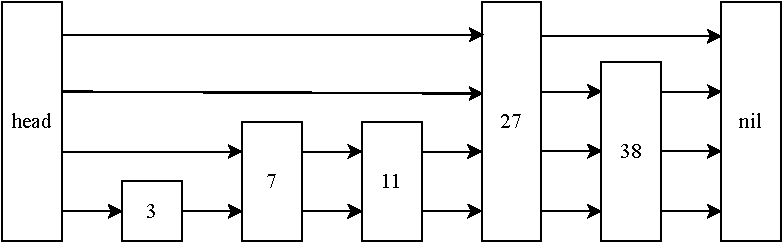
\includegraphics[width=.9\textwidth]{images/skiplist.pdf}
    \caption{Skiplist with 5 elements}
    \label{fig:skiplist}
\end{figure}

Searching in a skiplist can be summarised as follows. According to Pugh, starting at level $L(n) = \log_{1/p} n$ is most ideal, however, choosing level $0$ adds only a small constant to the complexity\cite{pugh-skiplist}. Starting at some level $n$, the key that we are searching for is compared to the key of the first forward pointer of the current node. In case the keys match, the node is found. In case the key is smaller than the next node's, we move a level down; else, we move one to the right. Until the node is found, or the current node points to nil, this procedure repeats. This algorithm is highlighted using dotted arrows in Figure \ref{fig:skip-search-insert}. 

\begin{figure}[!htb]
    \centering
    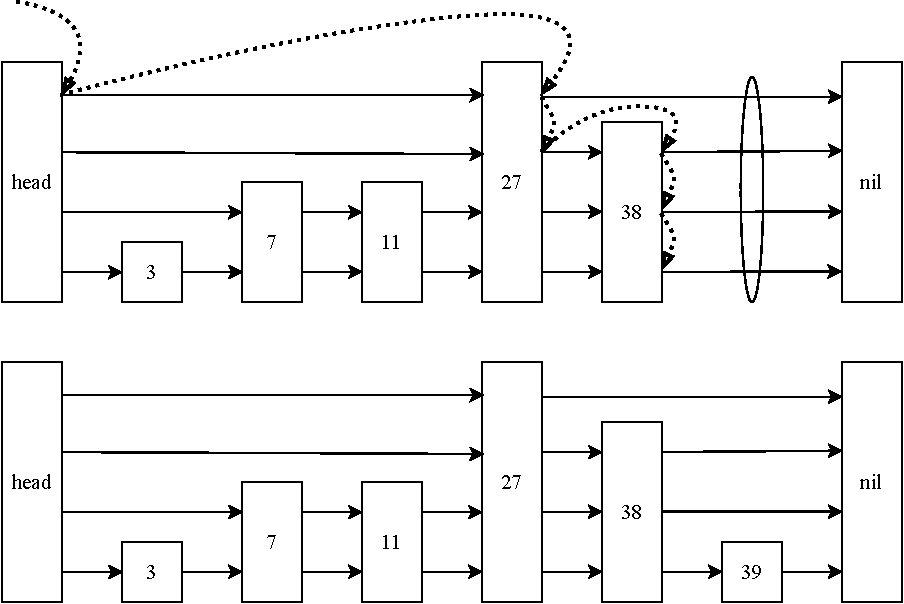
\includegraphics[width=.9\textwidth]{images/skip-search-insert.pdf}
    \caption{Inserting element $39$ with height $1$ into a skiplist. a) shows the search path to find the appropriate place on the last level. b) shows the final skiplist after insertion.}
    \label{fig:skip-search-insert}
\end{figure}

Inserting a key into a skiplist $L$, shown in Figure \ref{fig:skip-search-insert} and Algorithm \ref{alg:skip-insert}, consists of two parts. Firstly, on lines 1-8, the appropriate place of the new node needs to be found while also building an update list of pointers, which will be used to \textit{thread} the new node into the appropriate levels. Secondly, the new node needs to be inserted into the appropriate levels. If the node's random height is higher than the head's current one, the heads level is increased to match that of the new node. This is done on lines 11-17. Afterwards, a new node is allocated and threaded into the list. On line 20, the new nodes forward pointer at level $i$ is assigned the $i$th element's forward pointer in the update array. Finally, on line 21, the update array's $i$th element's forward pointers are pointed to the new node. 

\begin{algorithm}[!htb]
\caption{Skiplist-Insert(L, key)}
\label{alg:skip-insert}
\begin{algorithmic}[1]
    \State update $\gets$ [0..MaxLevel]
    \State x $\gets$ L.head
    \For{i $\gets$ L.level \textbf{downto} 0}
        \While{x.forward[i] $\neq$ nil $\land$ x.forward[i].key $<$ key}
            \State x $\gets$ x.forward[i]
        \EndWhile
        \State update[i] $\gets$ x
    \EndFor
    \State x $\gets$ x.forward[0]
    \If{x $=$ nil $\lor$ x.key $\neq$ key}
        \State h $\gets$ \Call{Get-Random-Height}{}()
        \If{h $>$ L.level}
            \For{i $\gets$ L.level$+1$ \textbf{to} h}
                \State update[i] $\gets$ L.head
            \EndFor
            \State L.level = h
        \EndIf
        \State n $\gets$ \Call{Create-Node}{h, key}
        \For{i $\gets$ 0 \textbf{to} level}
            \State n.forward[i] $\gets$ update[i].forward[i]
            \State update[i].forward[i] $\gets$ n
        \EndFor
    \EndIf
\end{algorithmic}
\end{algorithm}

Conceiving a lock-based or lock-free insertion algorithm into a skiplist would, much like with red-black trees, present a couple of difficulties that stem from the fact that the height of a node is not known in advance. A lock-based approach would need to figure out a cycle-free acquisition order of multiple node's forward pointers, and a lock-based approach would need to modify multiple locations at once when swinging the update array's forward pointers. This creates an unnatural and error-prone structure for the algorithms. Meanwhile, the transactional translation into C++, which shown in Figure \ref{fig:tx_skip_insert}, simplifies this into a naive sequential translation enclosed in a try-catch block which is retried until the transaction can commit. All reads are replaced with calls to \texttt{Tx.read()} and all writes are replaced with calls to \texttt{Tx.write()}.

\begin{figure}[!htb]
\begin{lstlisting}[language=C++]
template<class T>
void tx_skip_insert(Node<T> *n) {
    Transaction<> Tx;
    bool done = false;
    while (!done) {
        try {
            Tx.begin();
            Node<T> *curr = Tx.read(&head);
            Node<T> *update[MAX_LEVEL + 1];
            for (int i = Tx.read(&level); i >= 0; i--) {
                Node<T> *curr = Tx.read(&curr->neighbours[i]);
                while (curr && Tx.read(&curr->value) < n->value)
                    curr = Tx.read(&curr->neighbours[i]);
                update[i] = curr;
            }
            curr = Tx.read(&curr->neighbours[0]);
            if (!curr || Tx.read(&curr->value) != n->value) {
                int h = n->height;
                if (h > Tx.read(&level)) {
                    for (int i = Tx.read(&level)+1; i<h+1; i++)
                        update[i] = Tx.read(&head);
                    Tx.write(&level, h);
                }
                for (int i = 0; i <= h; i++) {
                    Tx.write(&n->neighbours[i], 
                             update[i]->neighbours[i]);
                    Tx.write(&update[i]->neighbours[i], n);
                }
            }
        }
        catch(AbortException&) {
            Tx.abort();
            done = false;
        }
    }
}
\end{lstlisting}
\caption{Transactional insertion into a Skiplist}
\label{fig:tx_skip_insert}
\end{figure}

Presented here the function \texttt{void tx\_skip\_insert(Node<T> *n)} is a member of the class \texttt{TransactionalSkiplist<T>} and is responsible for inserting a Node of type \texttt{T}.